\chapter{Theory}
\label{chp:theory}

\begin{center}
    \textit{This chapter delves into the theoretical foundations of the technologies and methodologies employed in the project. It covers key concepts such as computer vision, image recognition, and the integration of chess analysis tools like \Gls{stockfish}.}    
\end{center}

\section{Literature Review}
\label{sec:literature-review}

As technology continues to evolve, a variety of digital tools and platforms have emerged to enhance the experience of playing and analyzing chess. Leading online platforms such as \textit{chess.com} and \textit{lichess.org} provide global matchmaking, tutorials, and advanced game analysis features. These innovations have significantly transformed how chess is played and studied. \\

In parallel with these software-based innovations, physical chessboards and tournament practices have also been modernized through the integration of digital technologies. For instance, the use of \gls{rfid} enables the digitization of \gls{otb} games. \gls{rfid} works by embedding small tags in the chess pieces, which are detected by sensors in the board to identify each move \cite{quora:shah}. This approach bridges the gap between physical gameplay and digital analysis. \\

As an alternative to RFID-based systems, electronic scoresheet solutions have been introduced to enable digital recording of chess games. One notable example is Clono, a tablet-based platform that transmits move data directly to a central server. The system supports live of tournaments and offers a secure, low-cost and user-friendly interface. By removing the need for electronic chessboards, physical cables, or on-site technical staff, Clono presents a practical and accessible solution for modern tournament management. \cite{clono} \\

Advancements in \gls{ai} have also enabled the development of tools that automate the digitization of chess games through visual recognition. A prominent example is \textit{ChessCam}, a web- and mobile-based application that processes video footage or live streams to detect moves and generate \gls{pgn} files. This approach makes it possible to digitize games with minimal hardware and manual work. \cite{chess:chesscam, lichess:chesscam}

\section{Machine Learning} \label{sec:machine-learning}

As a subfield of \gls{ai}, \textbf{computer vision} focuses on enabling machines to interpret, analyze, and extract meaningful information from visual data, such as digital images and videos. The primary goal of computer vision is to replicate the human ability to perceive and understand visual information, as illustrated in Figure~\ref{fig:computer-vision}

\begin{figure}[h!] \centering 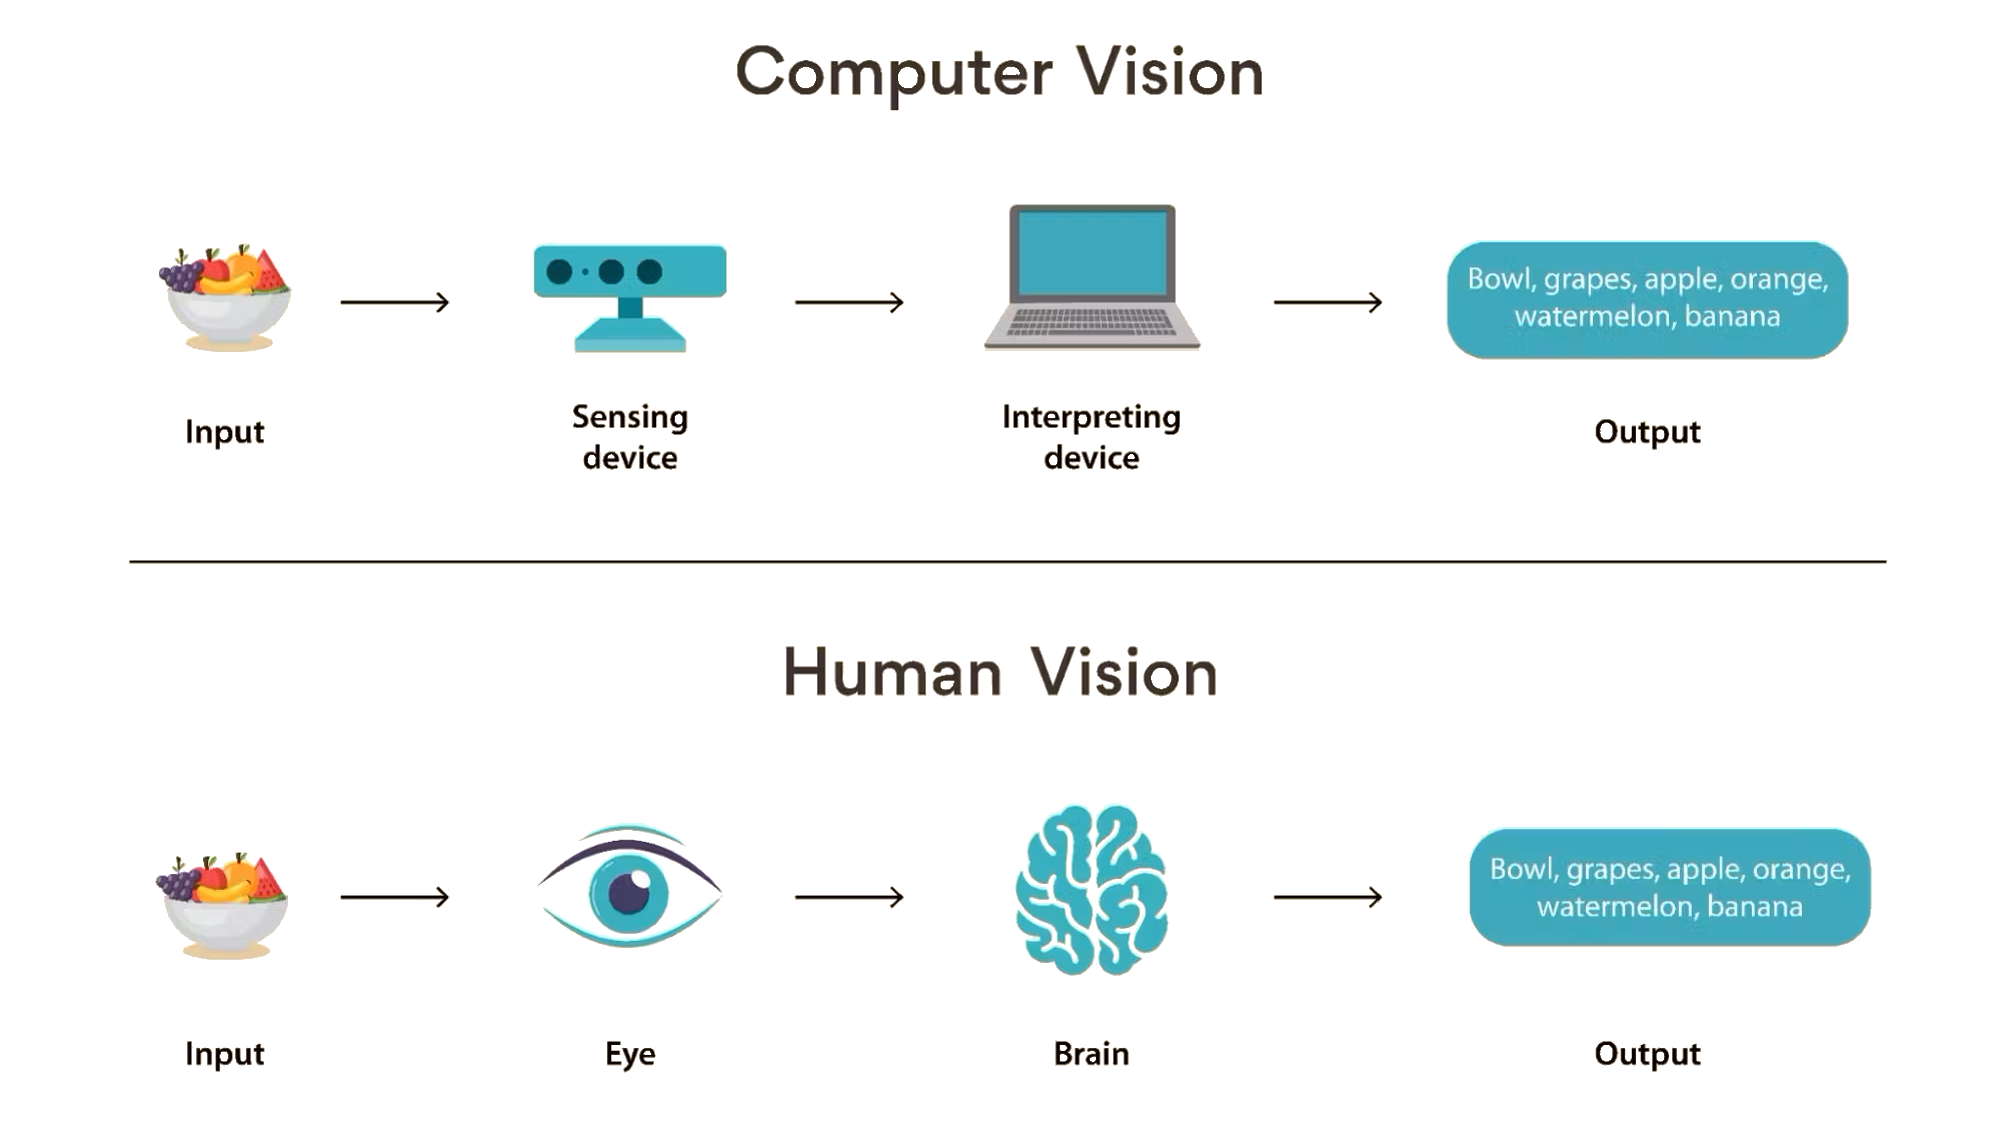
\includegraphics[width=0.75\linewidth]{figures/theory/machine-learning/computer-vision.png} \caption[Computer Vision vs. Human Vision]{Comparison of Computer Vision and Human Vision: Illustrating the similarities and differences in processing visual data \cite{turing:computer-vision}} \label{fig:computer-vision} \end{figure}

One of the most influential technologies in modern \gls{ml} is the \textbf{artificial neural network} (ANN). These networks excel at handling a wide range of data types, including images, audio, and text. Different neural network architectures are suited for specific tasks. For instance, recurring neural networks (RNNs), especially those incorporating \gls{lstm}, are effective for sequential data such as text. \\

In contrast, \textbf{\glspl{cnn}} are particularly effective in processing image data. Their architecture leverages convolutional layers to extract spatial features, making them highly efficient in image classification, object detection, and segmentation tasks. An example of such a network applied to handwritten digit classification is shown in Figure~\ref{fig:convolutional-neural-network}. \\

\newpage

\begin{figure}[h!] \centering 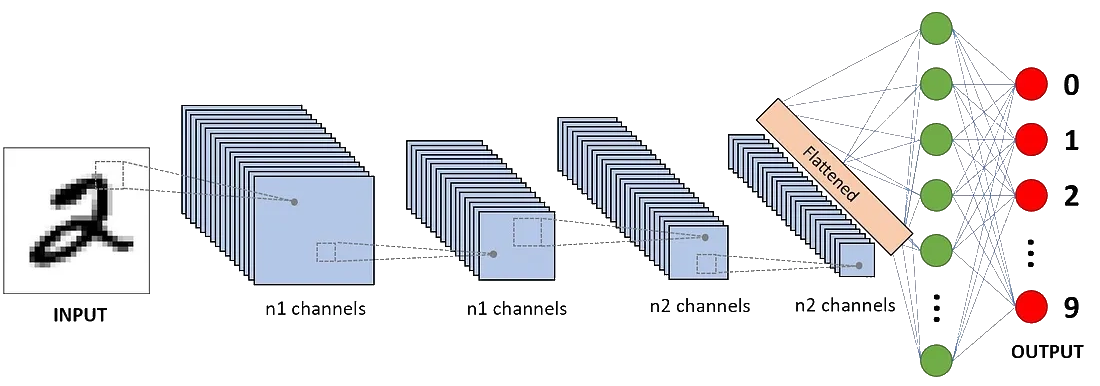
\includegraphics[width=0.75\linewidth]{figures/theory/machine-learning/convolutional-neural-network.png} \caption[Example of CNN architecture for handwritten digit classification]{CNN architecture for classifying handwritten digits \cite{medium:cnn}} \label{fig:convolutional-neural-network} \end{figure}


Due to their ability to learn hierarchical representations of visual data, CNNs have become a foundational tool in many computer vision applications, ranging from medical diagnostics to autonomous driving. Another fundamental concept in machine learning is \textbf{supervised learning}, where models are trained on labeled datasets. Each example in the dataset includes both an input and the correct output, allowing the model to learn how the input relates to the expected output. After training, the model can generalize this learned relationship to make predictions on new, unseen data \cite{geeksforgeeks:supervised-learning, google:supervised-learning}. \\

Within supervised learning, \textbf{classification} refers to predicting categorical outcomes. For example, a classification model trained on images of geometric shapes can learn to associate visual features with specific shape categories. When shown a new image, the model attempts to determine the most likely category based on its prior learning. This process is illustrated in Figure~\ref{fig:supervised-learning}, which shows how labeled data is used to train a model to make accurate predictions on unseen inputs. \\

\begin{figure}[h!] \centering 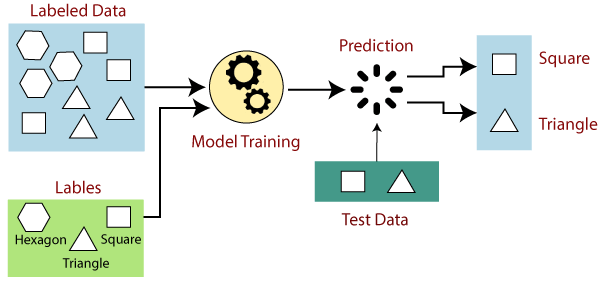
\includegraphics[width=0.75\linewidth]{figures/theory/machine-learning/supervised-learning.png} \caption[Supervised Learning with labeled data]{Supervised learning process using labeled data for classification \cite{tpointtech:supervised-learning}} \label{fig:supervised-learning} \end{figure}

By combining supervised learning with powerful models like CNNs, machine learning systems have achieved remarkable success in tasks that require human-like perception and decision-making [KILDE?]. As these models become more accurate and versatile, deploying them efficiently to real-world applications becomes increasingly important.  \\

To facilitate this, \textbf{\gls{onnx}} is an open-source format for representing machine learning models, enabling easy transfer and interoperability between different frameworks like PyTorch and TensorFlow \cite{roboflow:onnx}. \\

Similarly, \textbf{tensorflow} is an open-source machine learning framework developed by Google for building and deploying machine learning models. It provides comprehensive tools for deep learning, image processing, and natural language processing, and supports both training and inference of models \cite{nvidia:tensorflow}. \\

\textbf{Inference} refers to the process of using a trained machine learning model to make predictions on new, unseen data. In the context of object detection models, inference involves feeding an input image into the model, which then processes the image and outputs predictions. The predictions typically consist of object classes, confidence scores, and bounding box coordinates \cite{nvidia:inference}. \\

\section{Object Detection}

\textbf{\gls{leyolo}} is a \gls{cnn}-based architecturr designed for real-time object detection. It is a lightweight version of \gls{yolo} where its simplified architecture allows it to achieve significantly faster inference times. This makes it particularly suitable for real-time applications, where quick detection is more important than achieving the highest possible accuracy. Like its predecessor, it divides an image into a grid, and each cell predicts whether an object is present, along with its bounding box coordinates \cite{openreview:leyolo}.\\

Central to object detection is the use of concept of \textbf{bounding boxes}. Bounding boxes are rectangular regions used to indicate the location of an object within an image. It is typically represented by four values: the center coordinates \((x_c, y_c)\), which define the center of the box, and the width \((w)\) and height \((h)\), which define the dimensions of the box. In object detection tasks, models predict these coordinates to both localize and classify objects within an image \cite{peopleforai:boundingbox}. \\

\newpage

\begin{figure}[h!]
    \centering
    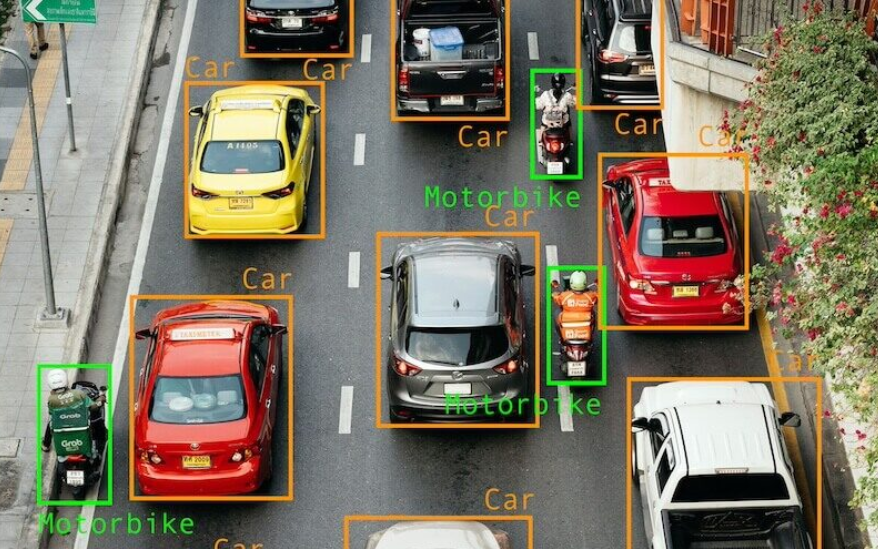
\includegraphics[width=0.75\linewidth]{figures/theory/image-recognition/bbox-example.png}
    \caption[Example of a bounding box in object detection]{Example of a bounding box used in object detection to localize an object within an image \cite{peopleforai:boundingbox}}
    \label{fig:boundingbox}
\end{figure}

To improve detection accuracy across different object sizes and shapes, models use \textbf{Anchor boxes}. Anchor boxes are predefined bounding boxes of various sizes and aspect ratios used as reference points for object detection models. These boxes are placed over the image or feature map to help the model predict the location and dimensions of objects. Rather than directly predicting bounding boxes, the model predicts offsets (shifts) relative to these anchor boxes, allowing it to adjust the box's position and size to fit the object. The model also predicts a confidence score indicating the likelihood that an object is present \cite{thinkautonomous:anchorboxes}.

\newpage

\begin{figure}[h!]
    \centering
    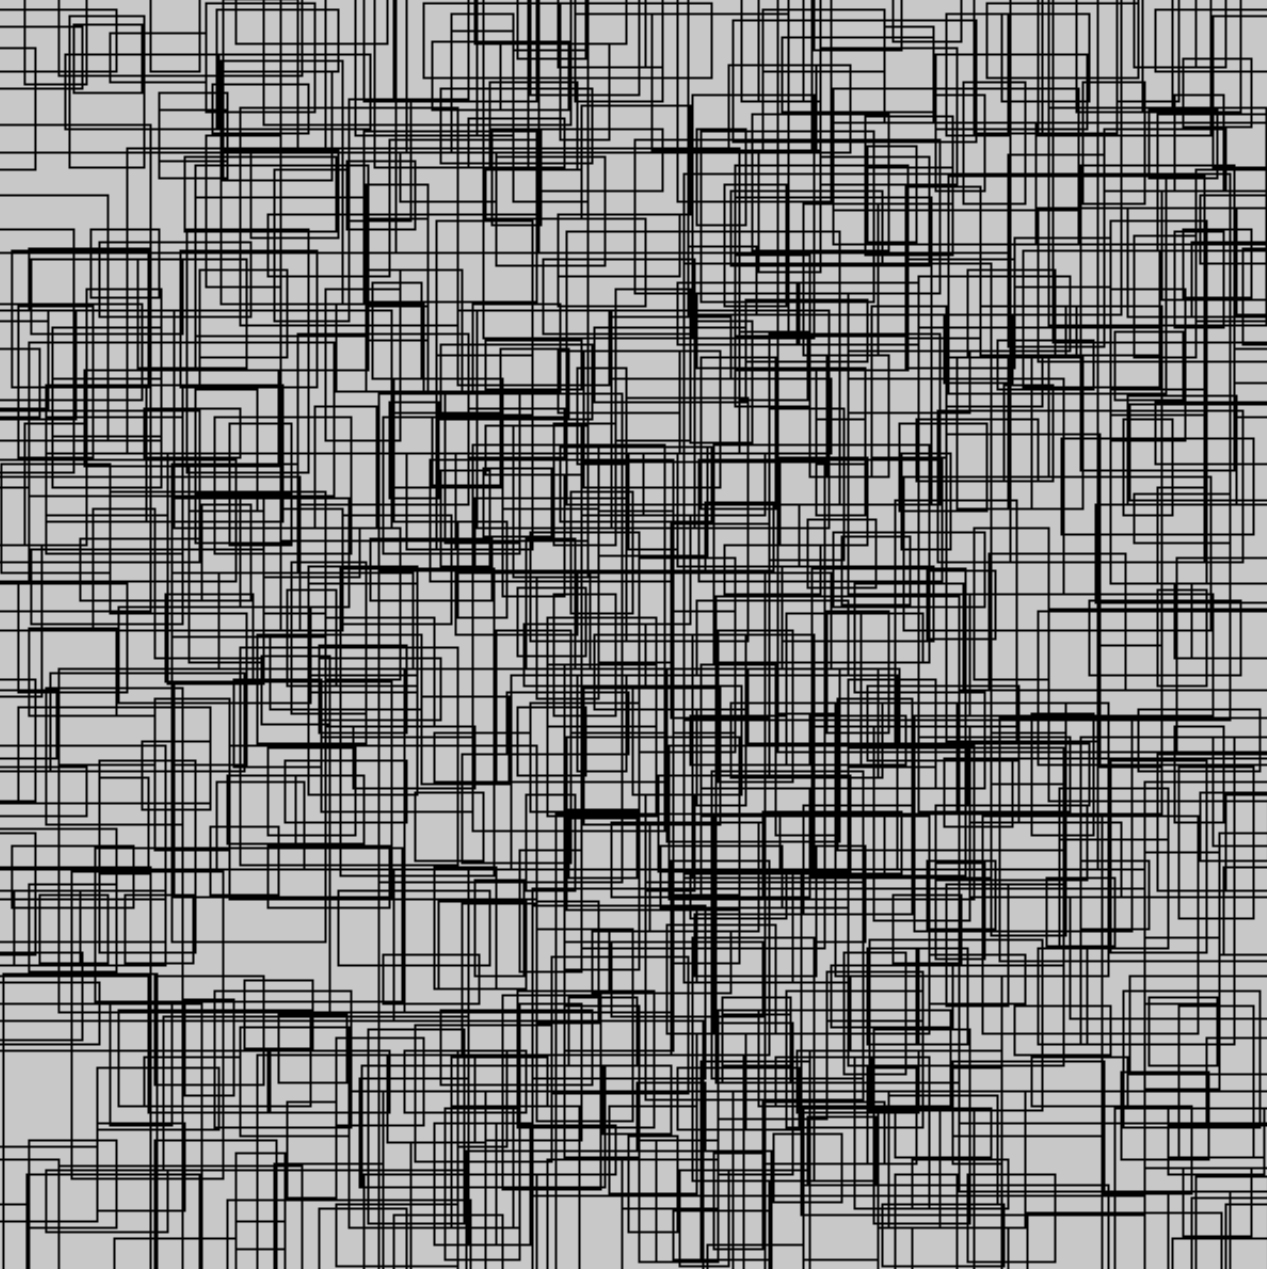
\includegraphics[width=0.7\linewidth]{figures/theory/image-recognition/anchor-boxes.png}
    \caption[Example of anchor boxes in object detection]{Illustration of multiple anchor boxes of different shapes and sizes centered on each grid cell in the image. These serve as initial reference boxes from which the model adjusts its predictions to fit actual objects
    \cite{thinkautonomous:anchorboxes}}
    \label{fig:anchor-box}
\end{figure}

 Once multiple predictions have been made, some of them may overlap significantly. To handle this, a post-processing technique called \textbf{\gls{nms}} is used. It removes redundant or overlapping bounding boxes and keeps only the most confident prediction. The NMS algorithm works by first selecting the box with the highest confidence score. It then removes all other boxes that have a high overlap with the selected box. This process is repeated iteratively until no boxes with significant overlap remain. By applying \gls{nms}, object detectors produce cleaner and more accurate results, preventing multiple detections of the same object
\cite{thepythoncode:nms}.

\newpage

\begin{figure}[h!]
    \centering
    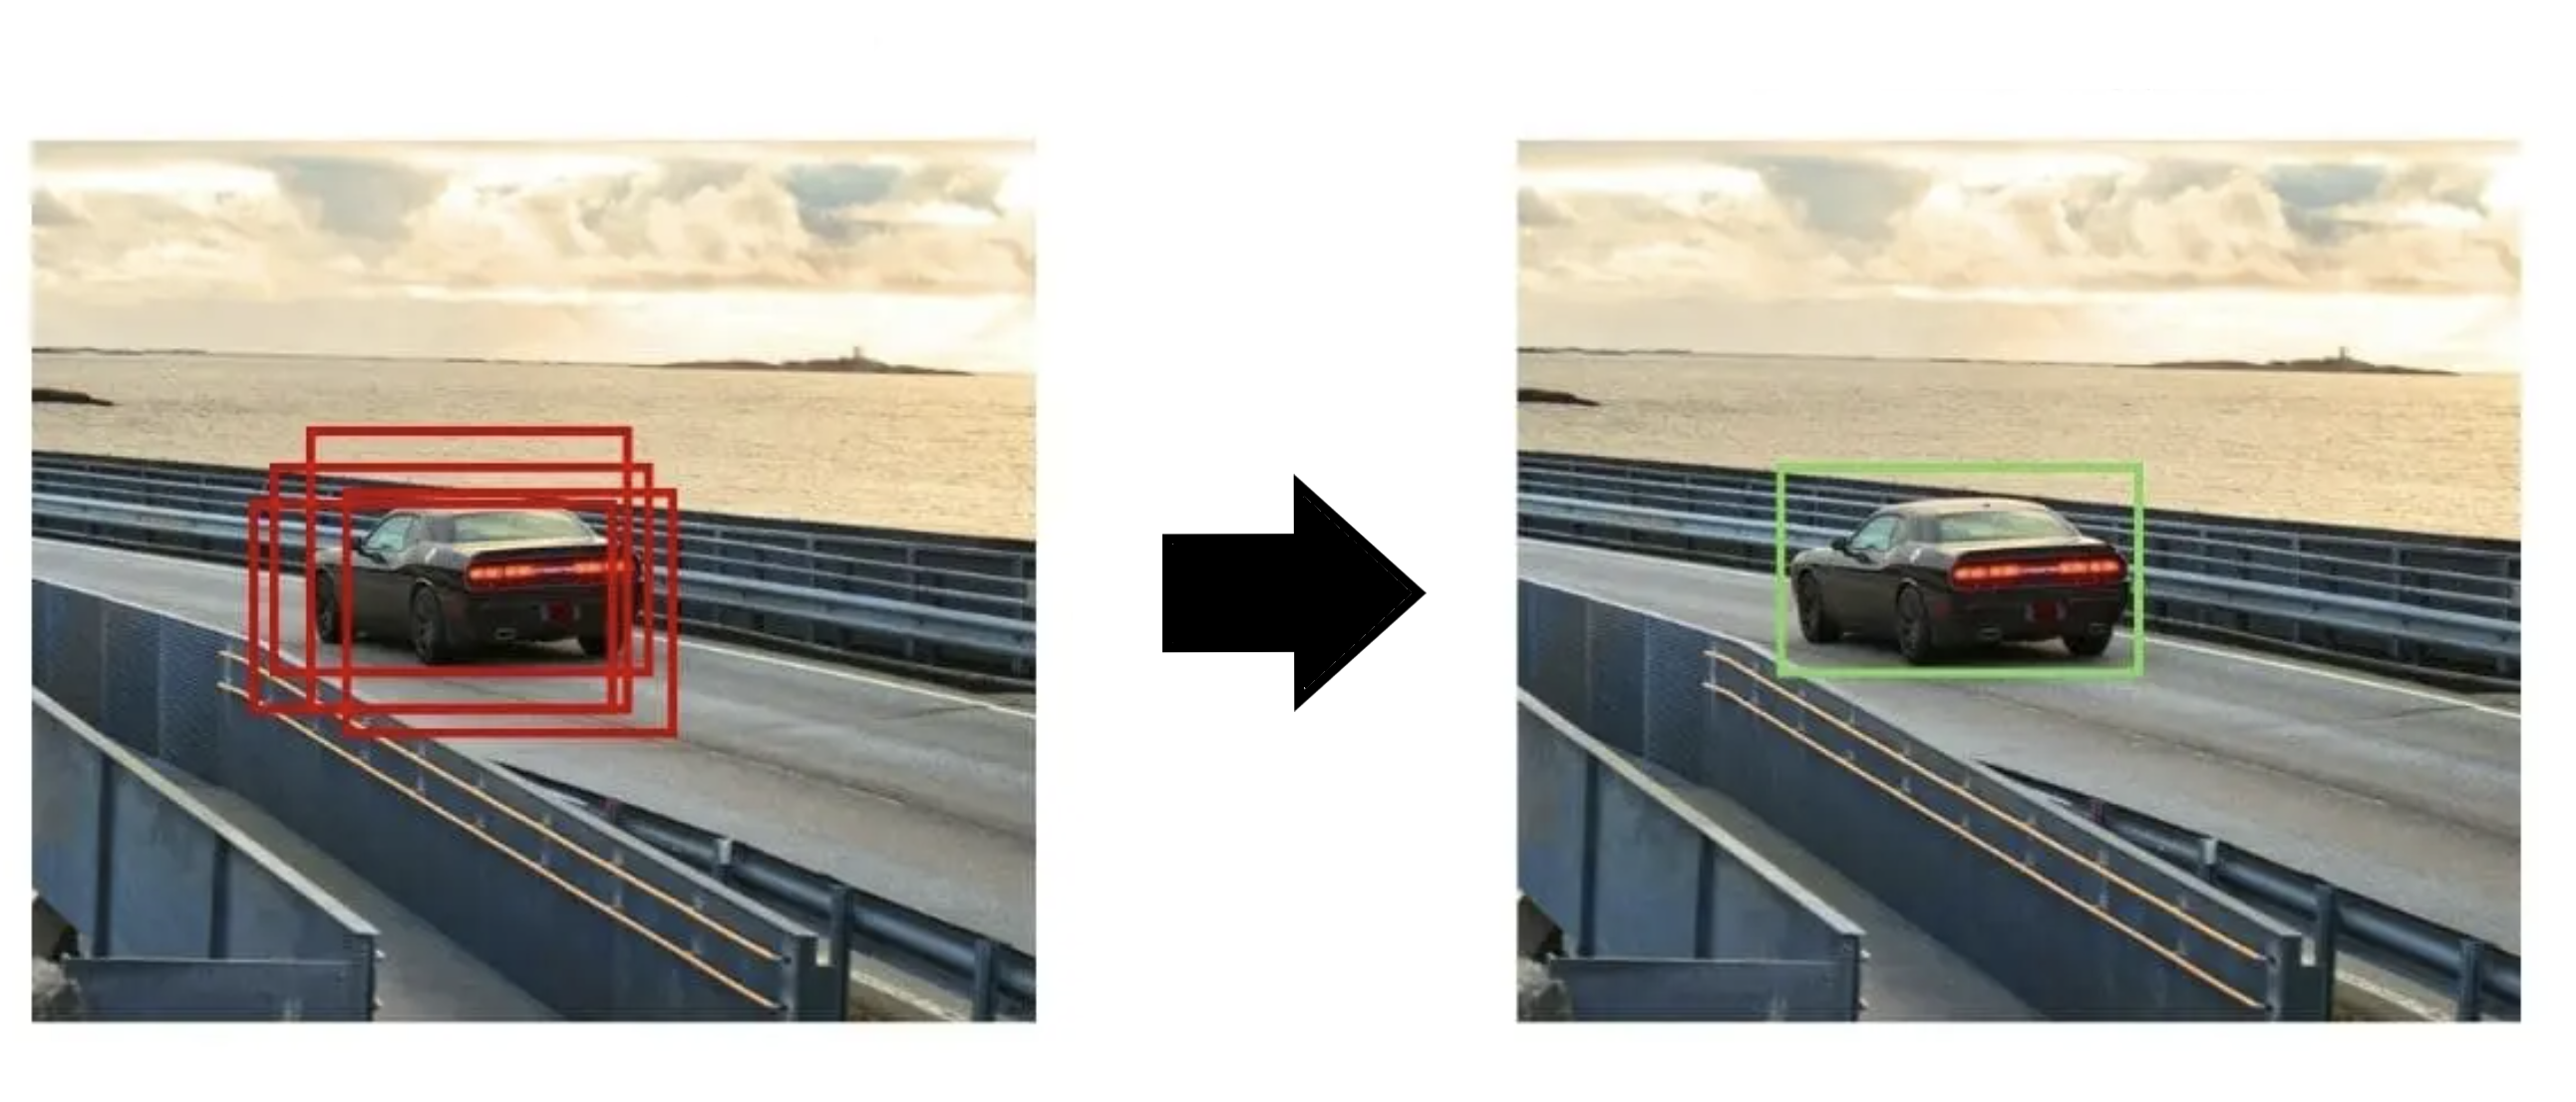
\includegraphics[width=0.75\linewidth]{figures/theory/image-recognition/nms.png}
    \caption[Non-maximum suppression (NMS) before and after applying the algorithm]{Illustration of NMS before and after its application. NMS retains the bounding box with the highest confidence score while suppressing those that significantly overlap with it \cite{thepythoncode:nms}}
    \label{fig:nms}
\end{figure}

\subsubsection*{Normalization}

Normalization in image processing involves scaling pixel values to a consistent range, typically [0, 1] or [-1, 1], to improve model performance. By adjusting pixel intensities from their original range (0-255) to a smaller scale, normalization ensures that the model processes inputs in a more stable and consistent manner. This accelerates model convergence. Normalization ensures that the input features are on a similar scale, aiding in more efficient and accurate learning.

\subsubsection*{Scaling}

Scaling in image processing and machine learning refers to transforming input data, such as images, to meet the specific requirements of a model. This typically involves resizing the image to a consistent size, normalizing pixel values to a standard range, and converting the image into the correct format expected by the model.





\begin{figure}[h!]
    \centering
    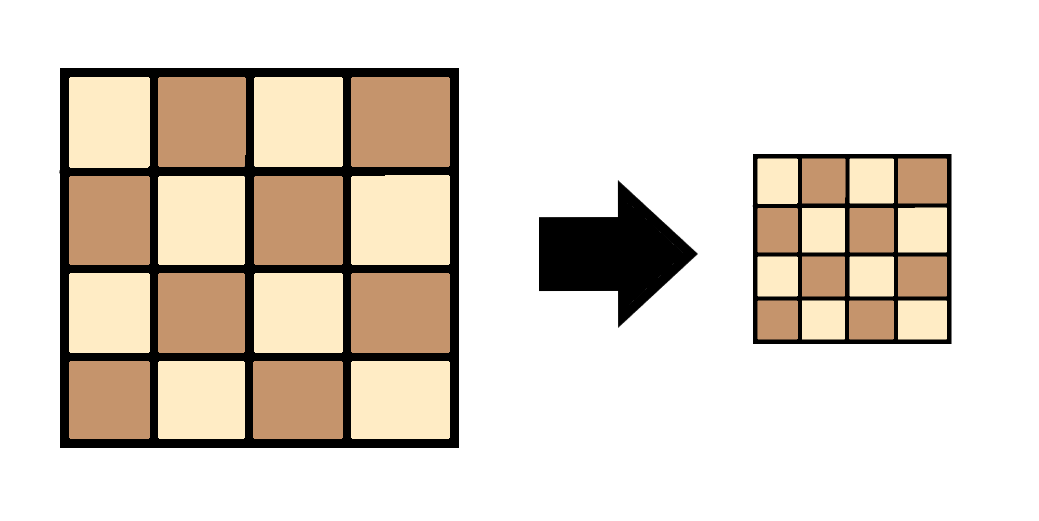
\includegraphics[width=0.75\linewidth]{figures/theory/image-recognition/scaling.png}
    \caption[Scaling process in image preprocessing]{Illustration of the scaling process in image preprocessing, resizing, normalizing, and converting the image format to prepare it for model input. \cite{thepythoncode:nms}}
    \label{fig:nms}
\end{figure}

Scaling process in image preprocessing]{Illustration of the scaling process in image preprocessing, including resizing, normalizing, and converting the image format to prepare it for model input.

\subsubsection*{Perspective Transformation}

When an image is taken from a tilted viewpoint, objects that are normally rectangular, such as a chessboard, appear distorted and no longer have right angles. A perspective transformation is a specific type of image warping that corrects distortions caused by viewing a flat object from an angle A perspective transformation uses mathematical techniques to map points from the distorted image back to their correct, undistorted positions \cite{nvidia:perspective-transform}.


\begin{figure}[h!]
    \centering
    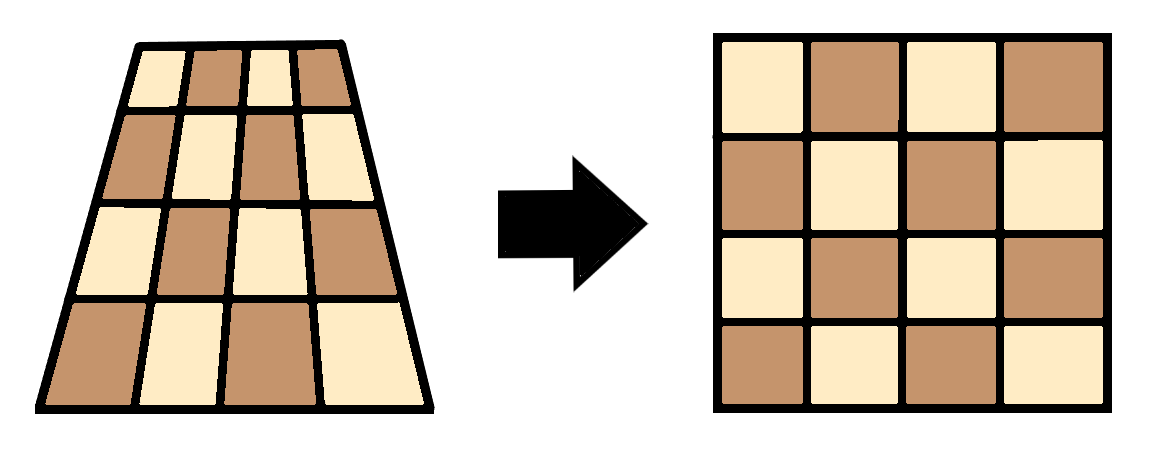
\includegraphics[width=0.75\linewidth]{figures/theory/image-recognition/perspective-transformation.png}
    \caption[Perspective transformation before and after]{Perspective transformation before and after applying the algorithm, demonstrating how distortion caused by an angled viewpoint is corrected to restore the object’s original shape.}
    \label{fig:perspective-transformation}
\end{figure}





The \textbf{Euclidean distance} is the straight-line distance between two points in a plane. For two points with coordinates $\mathbf{x} = (x_1, x_2)$ and $\mathbf{y} = (y_1, y_2)$, the Euclidean distance is given by:

\[
\sqrt{(x_2 - x_1)^2 + (y_2 - y_1)^2}
\]

As shown in Figure~\ref{fig:euclidean-distance}, the Euclidean distance represents the length of the straight line connecting the two points.

\begin{figure}[h!]
    \centering
    \fbox{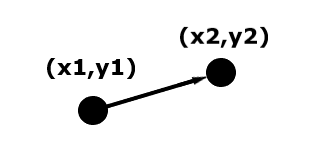
\includegraphics[width=0.4\linewidth]{figures/theory/math/euclidean-distance.png}}
    \caption{Illustration of Euclidean distance: the straight-line distance between two points in 2D space~\cite{geeksforgeeks:euclidean-distance}.}
    \label{fig:euclidean-distance}
\end{figure}




\section{Web}
\label{subsec:web}


\subsubsection*{Client-Server Architecture}
\label{subsubsec:client-server}

Client-server architecture is a network model in which multiple clients request and receive services from a centralized server over a local network or the Internet. Clients interact with the system through an application interface, while the server handles data processing. This architecture enables centralized control, scalability, and efficient resource management. See Figure~\ref{fig:client-server-architecture} \cite{liquidweb:client-server}.


\begin{figure}[h!]
    \centering
    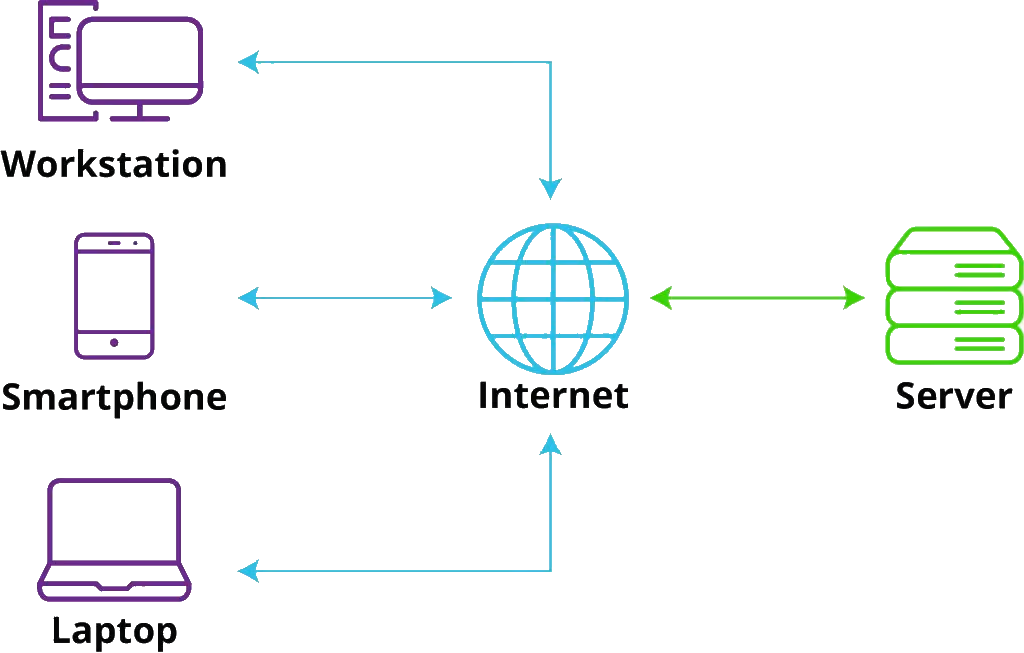
\includegraphics[width=0.75\linewidth]{figures/theory/client-server-architecture.png}
    \caption[Client-Server Architecture]{Client-Server Architecture \cite{liquidweb:client-server}}
    \label{fig:client-server-architecture}
\end{figure}

\subsubsection*{WebSocket}
\label{subsubsec:websocket}

WebSocket is a standardized communication protocol that enables full-duplex communication over a single \gls{tcp} connection, making it well-suited for real-time web applications. Unlike traditional \gls{http} requests — which follow a request-response model — WebSocket establishes a persistent connection that allows both the client and server to send and receive data at any time. This reduces the need for polling or long polling, significantly lowering network traffic and latency. As a result, WebSocket improves the efficiency and responsiveness of data transmission, particularly in applications such as live data feeds and online games. See Figure \ref{fig:websocket-vs-http} for a comparison \cite{nodejs:websocket, apidog:websocket}.


\begin{figure}[h!]
    \centering
    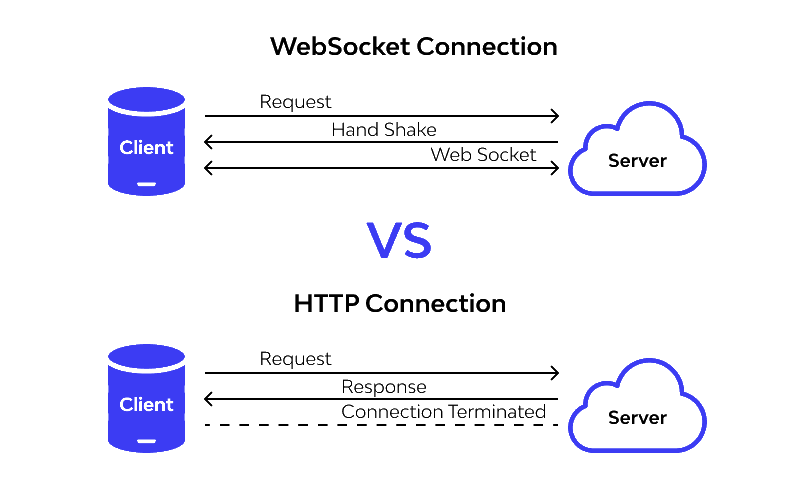
\includegraphics[width=0.75\linewidth]{figures/theory/websocket-vs-http.png}
    \caption[WebSocket Connection VS HTTP Connection]{WebSocket Connection VS HTTP Connection \cite{apidog:websocket}}
    \label{fig:websocket-vs-http}
\end{figure}

\section{Design}
\label{sec:design}

\subsection{Wireframe}
\label{subsec:wireframe}

A wireframe is a simplified visual representation of a user interface, used in the early stages of design to outline the structure and layout of a digital product. It focuses on functionality, content placement, and user interaction, without including detailed design elemens \cite{balsamiq:wireframe}.

subsection{WCAG}
\label{subsec:wcag}

The \gls{wcag} provide technical specifications to enhance the accessibility of websites and digital content. Developed by the World Wide Web Consortium (W3C), these guidelines aim to make digital experiences more accessible to individuals with various disabilities \cite{levelaccess:wcag}.

\section{Code Quality}
\label{sec:code-quality}

subsection{Code Review}
\label{subsec:code-review}

Code review is a process in which one or more developers examine another developer’s code before it is merged into a shared branch, such as the main branch. The purpose is to identify issues such as bugs, logic errors, or edge cases that may not have been caught during initial development \cite{gitlab:code-review}. //

Modern version control systems often use pull requests to facilitate code reviews. A pull request is a formal proposal to merge changes from one branch into another and provides a platform for reviewing, discussing, and approving code. It also highlights differences between branches, helping reviewers understand and evaluate the proposed changes \cite{github:pr}.

\subsection{Cohesion and Coupling}
\label{subsec:cohesion-and-coupling}

\begin{quote}
\textit{"\textbf{Cohesion} refers to the degree to which elements within a module work together to fulfill a single, well-defined purpose. \textbf{High cohesion} means that elements are closely related and focused on a single purpose, while \textbf{low cohesion} means that elements are loosely related and serve multiple purposes."} \cite{geeksforgeeks:c&c} \\
\end{quote}

\begin{quote}
\textit{"\textbf{Coupling} refers to the degree of interdependence between software modules. \textbf{Tight coupling} means that modules are closely connected and changes in one module may affect other modules. \textbf{Loose coupling} means that modules are independent, and changes in one module have little impact on other modules."} \cite{geeksforgeeks:c&c} \\
\end{quote}

\begin{figure}[h!]
    \centering
    \subfloat{{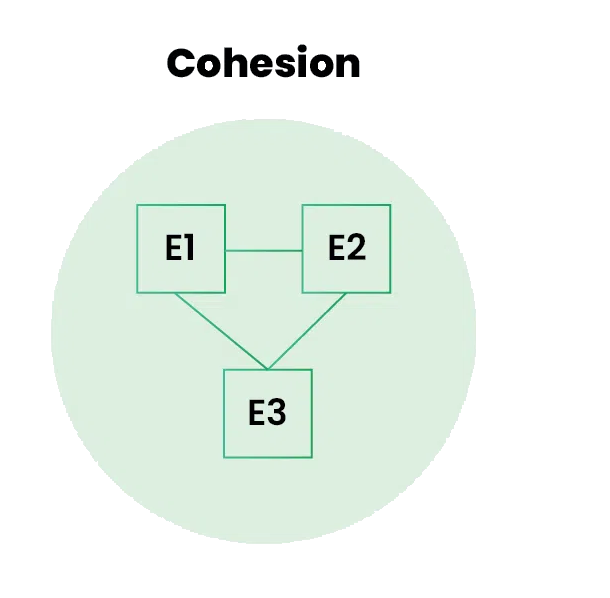
\includegraphics[width=0.5\linewidth]{figures/theory/cohesion.png}}}
    \subfloat{{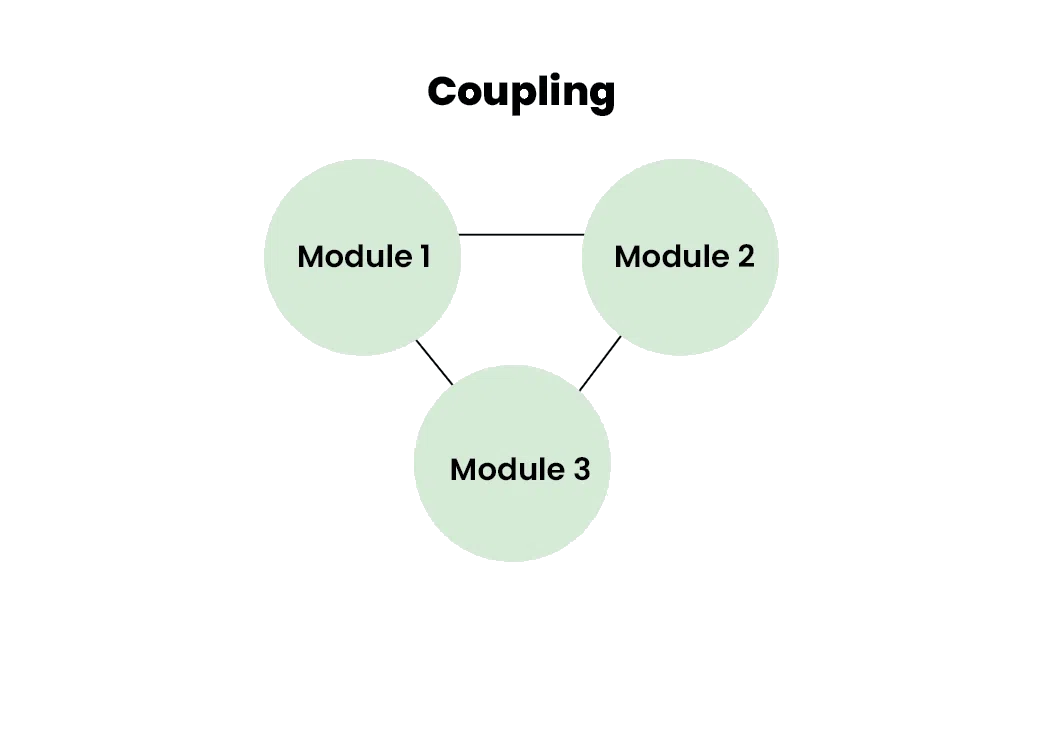
\includegraphics[width=0.5\linewidth]{figures/theory/coupling.png}}}

    \caption[Cohesion \& Coupling]{Cohesion \& Coupling \cite{geeksforgeeks:c&c}}
    \label{fig:cohesion-coupling}
\end{figure}

Cohesion and coupling significantly impact the quality and maintainability of a system.
High cohesion and loose coupling are desirable, as they lead to systems that are easier to test, modify, and extend. This relationship is illustrated in Figure \ref{fig:cohesion-coupling} 
\cite{geeksforgeeks:c&c}.

\subsection{Documentation}
\label{subsec:documentation}

Documentation is an essential part of software development, providing written references for developers, testers, and users. It includes materials such as \gls{api} references, build instructions, user guides, and design specifications. Documentation supports understanding, maintenance, and helps preserve knowledge over time. It should be created and maintained alongside the code to stay accurate and useful throughout the project lifecycle \cite{geeksforgeeks:doc}.

\subsection{Testing}
\label{subsec:testing}

\subsubsection*{Virtual Machine}
\label{subsubsec:virtual-machine}

A \gls{vm} is a software program that acts like a real computer. It runs on a physical machine (the host) and has its own virtual \gls{cpu}, memory, and storage. The VM is separated from the host system, so anything running inside the VM cannot directly affect the host. This makes it useful for testing, running different operating systems, or isolating software environments \cite{microsoft:virtual-machine}.

\subsubsection*{Unit Testing}
\label{subsubsec:unit-testing}

Unit testing involves testing individual components of a software application in isolation, such as functions, methods, or classes. The purpose is to ensure that each unit behaves as expected and is reliable under different conditions \cite{geeksforgeeks:unit-test}.

\subsubsection*{Usability Testing}
\label{subsec:usability-testing}

Usability testing evaluates a system from the end user’s perspective, focusing on how easily users can interact with the system to accomplish their goals. It involves observing users to identify areas of confusion, inefficiency, or difficulty in the user experience \cite{geeksforgeeks:user-test}.

Both qualitative data (e.g., user feedback) and quantitative data (e.g., task completion rates) are collected to assess functionality and user satisfaction. These findings are used to generate a report with recommendations for improving usability \cite{geeksforgeeks:user-test}.


\subsection{Type Safety}
\label{subsec:type-safety}

Type safety ensures that operations in a program are performed on the correct data types, helping catch errors early in development. In dynamically typed languages like JavaScript, lack of type enforcement can lead to hidden bugs. Enforcing type safety reduces runtime errors and improves code reliability \cite{dev:type-safety}.

\subsubsection*{Key Pillars of Type Safety}
\label{subsubsec:type-safety-pillars}

\begin{itemize}
\item \textbf{Reliability:} Enforcing correct data types prevents type-related runtime errors, improving application stability \cite{dev:type-safety}.

\item \textbf{Collaboration:} Clear type definitions make code easier to read and understand, aiding teamwork and maintainability \cite{dev:type-safety}.

\item \textbf{Efficient Debugging:} Detecting type errors early reduces debugging time and lowers the risk of runtime issues \cite{dev:type-safety}.
\end{itemize}
